\TUchapter{Attack Graph Generation}
\TUsection{Generation Algorithm}
\TUsection{Alternatives}
\TUsection{Example}
In order to aid understanding the generation process, this section  demonstrates a
sample attack graph generation process using an example. The reader is warned to
avoid searching for meaning or design in the selection of these assets, qualities,
and topologies; they are intended to be illustrative only, and any relation to 
real world networks, problems, attacks, or situations is purely coincidental.
This section will use the network model specification in Fig.~\ref{fig:ill_nm}
and the exploit patterns in Fig.~\ref{fig:ill_xp}.
\begin{figure}
\begin{lstlisting}
network model = 
    assets :
        asset_1;
        asset_2;
        asset_3;

    facts :
        quality:asset_1,quality_1=value_1;
        quality:asset_2,quality_1=value_2;
        quality:asset_3,quality_1=value_1;
        topology:asset_1->asset_2,topology_1;
        topology:asset_3->asset_2,topology_1;
.
\end{lstlisting}
\label{fig:ill_nm}
\end{figure}

\begin{figure}
\begin{lstlisting}
exploit exploit_1(asset_param_1,asset_param_2)=
    preconditions:
        quality:asset_param_1,quality_1=value_1;
        topology:asset_param_1->asset_param_2,topology_1;
    postconditions:
        delete topology:asset_param_1->asset_param_2,topology_1;
        insert topology:asset_param_2->asset_param_1,topology_1;
.

exploit exploit_2(asset_param_1,asset_param_2)=
    preconditions:
        quality:asset_param_1,quality_1=value_2;
        topology:asset_param_1->asset_param_2,topology_1;
    postconditions:
        insert quality:asset_param_2,quality_1=value_2;
.
\end{lstlisting}
\label{fig:ill_xp}
\end{figure}

Fig.~\ref{fig:ill_topology_0} represents the initial network state 
(denoted State 0) specified
in this example. Note that Fig.~\ref{fig:ill_topology_0} is \emph{not} an attack
graph, merely a convenient graph based representation of the example network
in use here. Each node represents an asset in the network state; it is labeled
first with the state number (in this case 0) and the asset name, then with a
listing of its qualities (in this case, there is only one).
Likewise, the edges that represent topologies
are labeled with the topology name they represent.

\begin{figure}
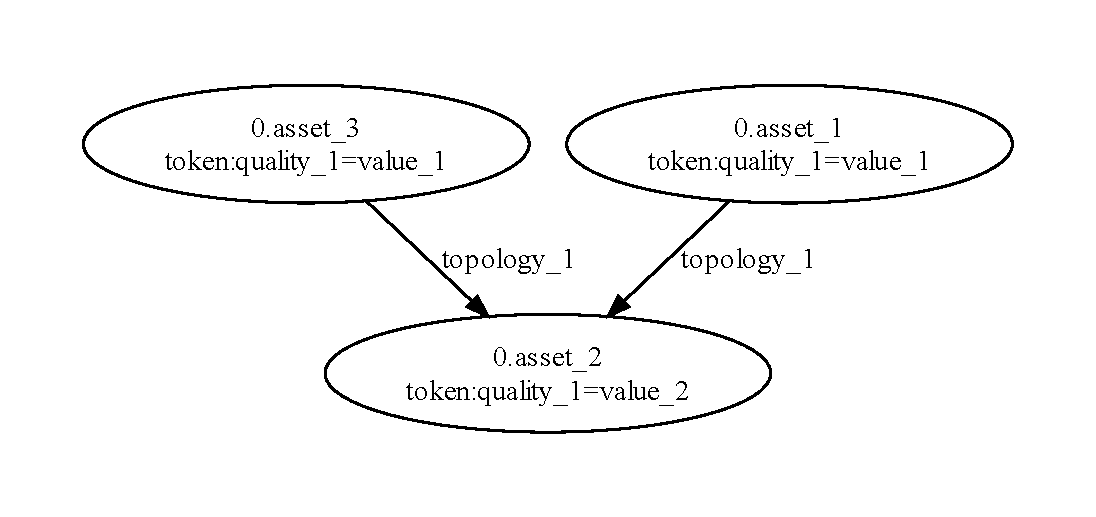
\includegraphics[width=4in]{ag_illustrative_simple/nm_state0}
\label{fig:ill_topology_0}
\end{figure}

Execution of the generation process begins by specifying a maximum ``depth''
of generation, which will be 2 for the purposes of this exercise, and by creating
an initial list of states for analysis, which contains only State 0.

Generation of the next set of states begins by creating a list of all valid
attacks on State 0; that is, selecting all valid bindings of assets given State 0's
fact base to exploit pattern parameters given their preconditions. Two such bindings
are possible from State 1: \texttt{exploit\_1(asset\_1, asset\_2)}; and 
\texttt{exploit2(asset\_3, asset\_2)}. Both bindings result in new states:
State 1 (Fig.~\ref{fig:ill_topology_1}) and State 2 (Fig.~\ref{fig:ill_topology_2}.
This completes a single execution of the generation function; although the leaves
are yet to be analyzed, a small attack graph is already the result 
(Fig.~\ref{fig:ill_ag_depth1}).

\begin{figure}
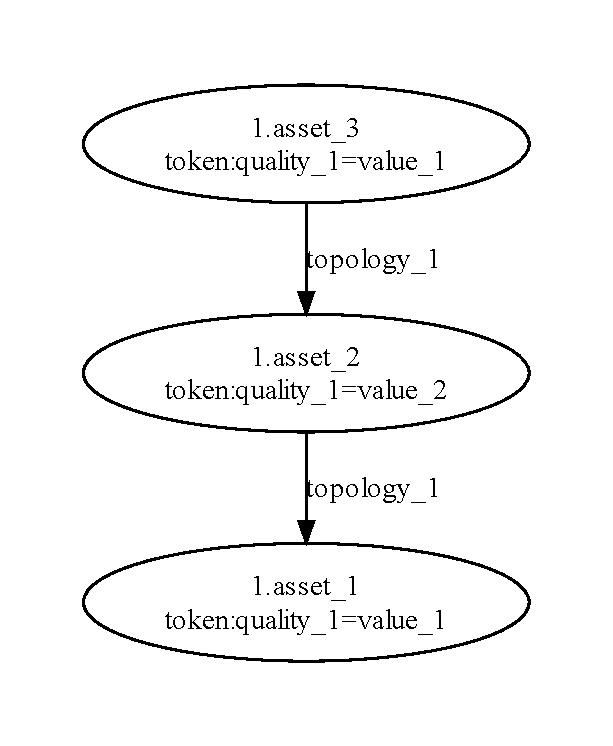
\includegraphics[width=4in]{ag_illustrative_simple/nm_state1}
\caption{State 1 of the illustrative discrete example}
\label{fig:ill_topology_1}
\end{figure}

\begin{figure}
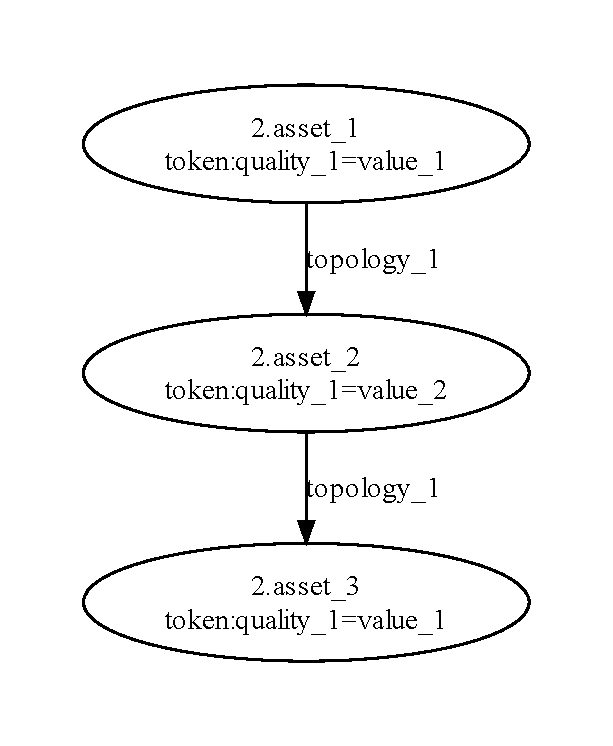
\includegraphics[width=4in]{ag_illustrative_simple/nm_state2}
\caption{State 2 of the illustrative discrete example}
\label{fig:ill_topology_2}
\end{figure}

\begin{figure}
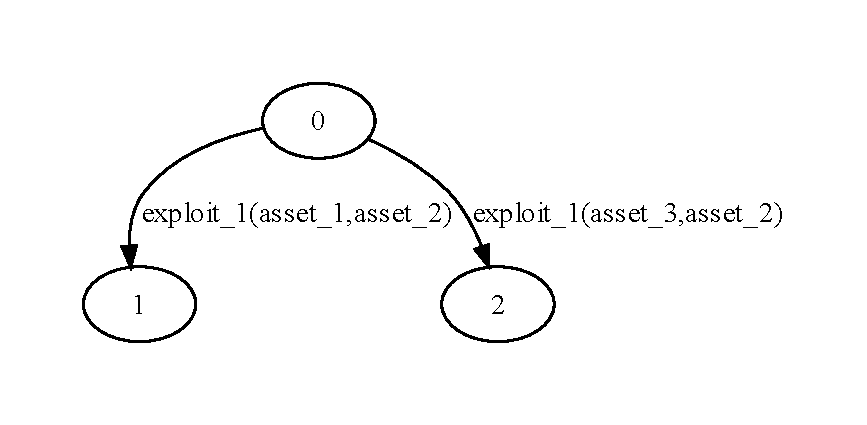
\includegraphics[width=4in]{ag_illustrative_simple/ag_depth1}
\caption{Attack graph after first iteration}
\label{fig:ill_topology_2}
\end{figure}

For the next execution of the generation function, the successor state list becomes
the new analysis state list, consisting now only of State 2, and the 
remaining allowed ``depth'' is decremented to 2. 6 attacks are possible from State 2:
\texttt{exploit\_2(asset\_1, asset\_2)}, \texttt{exploit\_2(asset\_2, asset\_1)}, 
\texttt{exploit\_2(asset\_1, asset\_3)}, \texttt{exploit\_2(asset\_3, asset\_1)},
\texttt{exploit\_2(asset\_2, asset\_3)}, and \texttt{exploit\_2(asset\_3, asset\_2)}. The process
iterates through these attacks, generating new states and, if they are new, adding them
to the list of successor states. \texttt{exploit\_2(asset\_1, asset\_2)} results in a new
state, State 3 (see Fig.~\ref{fig:ill_topology_3}), which is added to the list of
successor states. \texttt{exploit\_2(asset\_2, asset\_1)} also results in State 3, which
already exists and is therefore not added to the list of successor states. 
\texttt{exploit\_2(asset\_1, asset\_3)} generates a new state, State 4 
(see Fig.~\ref{fig:ill_topology_4}), which is added to the list of successor states.
\texttt{exploit\_2(asset\_3, asset\_1)} also generates State 4.
\texttt{exploit\_2(asset\_2, asset\_3)} and \texttt{exploit\_2(asset\_3, asset\_2)}
both result in State 2, which exists and is not added to the successor states.

\begin{figure}
\centering
\begin{dot2tex}[options=-t raw --autosize]
digraph G {
    rankdir=LR;
    asset_1 [shape=circle, texlbl="\begin{tabular}{c}\texttt{\bf asset\_1} \\ $2$ \end{tabular}"];
    asset_2 [shape=circle, texlbl="\begin{tabular}{c}\texttt{\bf asset\_2} \\ $2$ \end{tabular}"];
    asset_3 [shape=circle, texlbl="\begin{tabular}{c}\texttt{\bf asset\_3} \\ $2$ \end{tabular}"];
    asset_2 -> asset_3 [label=" ", texlbl="2"];
    asset_1 -> asset_2 [label=" ", texlbl="2"];
    
    asset_3 -> asset_2 [label=" ", texlbl="2"];
    asset_2 -> asset_1 [label=" ", texlbl="2"];
}
\end{dot2tex}
\caption{State 3 of the illustrative discrete example}
\label{fig:ill_topology_3}
\end{figure}

\begin{figure}
\centering
\begin{dot2tex}[options=-t raw --autosize]
digraph G {
    rankdir=LR;
    asset_1 [shape=circle, texlbl="\begin{tabular}{c}\texttt{\bf asset\_1} \\ $2$ \end{tabular}"];
    asset_2 [shape=circle, texlbl="\begin{tabular}{c}\texttt{\bf asset\_2} \\ $2$ \end{tabular}"];
    asset_3 [shape=circle, texlbl="\begin{tabular}{c}\texttt{\bf asset\_3} \\ $2$ \end{tabular}"];
    asset_2 -> asset_3 [label=" ", texlbl="2"];
    asset_1 -> asset_3 [label=" ", texlbl="2"];
    
    asset_3 -> asset_2 [label=" ", texlbl="2"];
    asset_3 -> asset_1 [label=" ", texlbl="2"];
}
\end{dot2tex}
\caption{State 4 of the illustrative discrete example}
\label{fig:ill_topology_4}
\end{figure}

The next iteration finds the remaining allowed depth at 1 and the list of
analysis states to contain State 3 and State 4. From State 3, the
possible attacks are the same as the possible attacks in State 2:
\texttt{exploit\_2(asset\_1, asset\_2)}, \texttt{exploit\_2(asset\_2, asset\_1)},
\texttt{exploit\_2(asset\_1, asset\_3)}, \texttt{exploit\_2(asset\_3, asset\_1)},
\texttt{exploit\_2(asset\_2, asset\_3)}, and \texttt{exploit\_2(asset\_3, asset\_2)}.
Only the middle two, \texttt{exploit\_2(asset\_1, asset\_3)}, \texttt{exploit\_2(asset\_3, asset\_1)},
generate a state that is not State 3 itself: State 5 (see Fig.~\ref{fig:ill_topology_5}),
which is added to the list of successor states. The rest simply create new reflexive
edges on State 3. The list of possible attacks on State 4 is the same, with only
\texttt{exploit\_2(asset\_1, asset\_2)} and \texttt{exploit\_2(asset\_2, asset\_1)} generating
a state other than State 4 itself. Both of those attacks generate State 5 again, which
already exists and therefore is not added to the list of successor states.

\begin{figure}
\centering
\begin{dot2tex}[options=-t raw --autosize]
digraph G {
    rankdir=LR;
    asset_1 [shape=circle, texlbl="\begin{tabular}{c}\texttt{\bf asset\_1} \\ $2$ \end{tabular}"];
    asset_2 [shape=circle, texlbl="\begin{tabular}{c}\texttt{\bf asset\_2} \\ $2$ \end{tabular}"];
    asset_3 [shape=circle, texlbl="\begin{tabular}{c}\texttt{\bf asset\_3} \\ $2$ \end{tabular}"];
    asset_1 -> asset_2 [label=" ", texlbl="2"];
    asset_2 -> asset_3 [label=" ", texlbl="2"];
    asset_3 -> asset_1 [label=" ", texlbl="2"];
    
    asset_2 -> asset_1 [label=" ", texlbl="2"];
    asset_3 -> asset_2 [label=" ", texlbl="2"];
    asset_1 -> asset_3 [label=" ", texlbl="2"];
}
\end{dot2tex}
\caption{State 5 of the illustrative discrete example}
\label{fig:ill_topology_5}
\end{figure}

The next iteration finds the list of analysis states to contain only State 5, and
the remaining allowed depth is 0. Because the depth limit is reached, generation
ceases. However, even if the depth limit had not been reached, execution would have
soon terminated. All 6 possible attacks from State 5 would have generated State 5 itself.
Therefore the list of successor states would be empty, and the next iteration's list of
analysis states would be empty, which would also cause generation to cease. A representation
of the resulting attack graph (with execution halting after 3 iterations) is provided
in Fig.~\ref{fig:ill_attack_graph}.

\begin{figure}
\centering
\begin{dot2tex}[options=-t raw --autosize]
digraph G {
    rankdir=LR;
    state_1 [shape=circle, texlbl="State 1"];
    state_2 [shape=circle, texlbl="State 2"];
    state_3 [shape=circle, texlbl="State 3"];
    state_4 [shape=circle, texlbl="State 4"];
    state_5 [shape=circle, texlbl="State 5"];
    
    state_1 -> state_1;
    state_1 -> state_1;
    state_1 -> state_2;
    
    state_2 -> state_2;
    state_2 -> state_2;
    state_2 -> state_3;
    state_2 -> state_3;
    state_2 -> state_4;
    state_2 -> state_4;
    
    state_3 -> state_3;
    state_3 -> state_3;
    state_3 -> state_3;
    state_3 -> state_3;
    state_3 -> state_5;
    state_3 -> state_5;
    
    state_4 -> state_4;
    state_4 -> state_4;
    state_4 -> state_4;
    state_4 -> state_4;
    state_4 -> state_5;
    state_4 -> state_5;
}
\end{dot2tex}
\caption{The illustrative example's attack graph to depth 3}
\label{fig:ill_attack_graph}
\end{figure}

This concludes the description of the basic attack graph model employed at the
University of Tulsa. The chapters following this one are devoted to
this model's expansion and analysis.